% Standalone XeLaTeX source. Uses standard commands and distributed packages.
% Source problem: public/notes/物工/問題/2011ap_exam.pdf, PDF page 2.
\documentclass[11pt,a4paper]{article}
\usepackage[margin=24mm]{geometry}
\usepackage{fontspec}
\usepackage{xeCJK}
\setCJKmainfont{HaranoAjiMincho-Regular.otf}
\setCJKsansfont{HaranoAjiGothic-Medium.otf}
\usepackage{amsmath,amssymb}
\usepackage{tikz}
\usetikzlibrary{arrows.meta,angles,quotes}
\setlength{\parindent}{1em}
\setlength{\parskip}{0.35em}
\renewcommand{\figurename}{図}
\title{物理工学専攻 院試解答集 ver2\\2011年 物理学I 第1問}
\author{政岡凜太郎}
\date{}
\begin{document}
\maketitle

\section*{幾何と記号}
円板の中心を原点$O$、糸の固定端を$A=(a,0)$とする。
円板と糸の接点を$Q$とし、$OQ$が正の$x$軸となす反時計回りの角を$\varphi$とする。
糸が伸びず、円板に沿って巻きつくので、円板上の糸の長さは$a\varphi$である。
したがって、$Q$から質点までの自由な糸の長さは
\begin{equation}
  \ell(\varphi)=\ell_0-a\varphi
  \label{eq:length}
\end{equation}
となる。以下は衝突前の$\ell>0$に対する議論である。
半径方向と接線方向の単位ベクトルを
\begin{equation}
  \boldsymbol{e}_r=\begin{pmatrix}\cos\varphi\\\sin\varphi\end{pmatrix},
  \qquad
  \boldsymbol{e}_{\varphi}=\begin{pmatrix}-\sin\varphi\\\cos\varphi\end{pmatrix}
\end{equation}
と定める。自由な糸は$Q$から$\boldsymbol{e}_{\varphi}$の方向に伸び、張力はその逆方向に働く。

\begin{figure}[htbp]
\centering
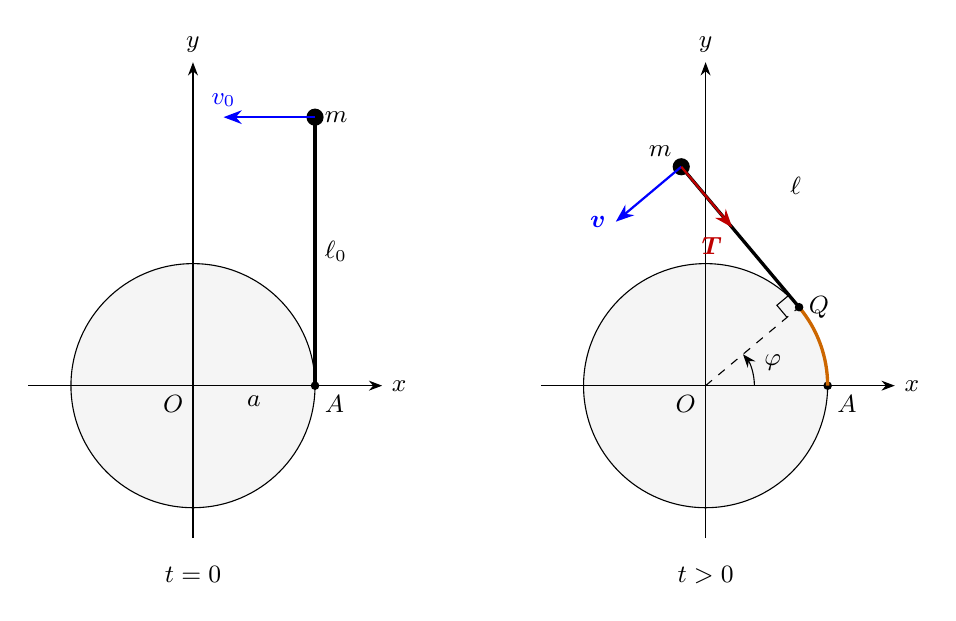
\begin{tikzpicture}[scale=1.55,>=Stealth,font=\small]
  \pgfmathsetmacro{\radius}{1}
  \pgfmathsetmacro{\ellZero}{2.2}
  \pgfmathsetmacro{\phiAngle}{40}
  \pgfmathsetmacro{\phiRadians}{\phiAngle*pi/180}
  \pgfmathsetmacro{\freeLength}{\ellZero-\radius*\phiRadians}
  \begin{scope}[xshift=-2.1cm]
    \draw[fill=gray!8] (0,0) circle (\radius);
    \draw[->] (-1.35,0)--(1.55,0) node[right] {$x$};
    \draw[->] (0,-1.25)--(0,2.65) node[above] {$y$};
    \node[below left] at (0,0) {$O$};
    \fill (\radius,0) circle (1pt) node[below right] {$A$};
    \draw[very thick] (\radius,0)--(\radius,\ellZero);
    \fill (\radius,\ellZero) circle (2pt) node[right] {$m$};
    \draw[->,blue,thick] (\radius,\ellZero)--(\radius-0.75,\ellZero) node[above] {$v_0$};
    \node[right] at (\radius,\ellZero/2) {$\ell_0$};
    \node[below] at (\radius/2,0) {$a$};
    \node at (0,-1.55) {$t=0$};
  \end{scope}
  \begin{scope}[xshift=2.1cm]
    \coordinate (O) at (0,0);
    \coordinate (A) at (\radius,0);
    \coordinate (Q) at ({\radius*cos(\phiAngle)},{\radius*sin(\phiAngle)});
    \coordinate (P) at ({\radius*cos(\phiAngle)-\freeLength*sin(\phiAngle)},
                         {\radius*sin(\phiAngle)+\freeLength*cos(\phiAngle)});
    \draw[fill=gray!8] (0,0) circle (\radius);
    \draw[->] (-1.35,0)--(1.55,0) node[right] {$x$};
    \draw[->] (0,-1.25)--(0,2.65) node[above] {$y$};
    \node[below left] at (O) {$O$};
    \fill (A) circle (1pt) node[below right] {$A$};
    \draw[very thick,orange!80!black] (A) arc[start angle=0,end angle=\phiAngle,radius=\radius];
    \draw[dashed] (O)--(Q);
    \fill (Q) circle (1pt) node[right] {$Q$};
    \draw[very thick] (Q)--(P) node[midway,above right,xshift=5mm,yshift=4mm] {$\ell$};
    \fill (P) circle (2pt) node[above left] {$m$};
    \draw[->,blue,thick] (P)--++({-0.7*cos(\phiAngle)},{-0.7*sin(\phiAngle)}) node[left] {$\boldsymbol{v}$};
    \draw[->,red!75!black,thick] (P)--++({0.65*sin(\phiAngle)},{-0.65*cos(\phiAngle)}) node[below left] {$\boldsymbol{T}$};
    \draw[->] (0.4*\radius,0) arc[start angle=0,end angle=\phiAngle,radius=0.4*\radius];
    \node at (0.55,0.19) {$\varphi$};
    \pic[draw,angle radius=2mm] {right angle=O--Q--P};
    \node at (0,-1.55) {$t>0$};
  \end{scope}
\end{tikzpicture}
\caption{左は初期状態、右は巻きつく途中の模式図。右の速度は$-\boldsymbol{e}_r$方向、張力は$-\boldsymbol{e}_{\varphi}$方向を向く。太い弧は巻きついた糸を表す。表示例では $\varphi=40^\circ$、$\ell_0/a=2.2$ とし、寸法比の予測には用いない。}
\label{fig:geometry}
\end{figure}

\section*{[1] エネルギーと角運動量の保存}
位置は$\boldsymbol{r}=a\boldsymbol{e}_r+\ell\boldsymbol{e}_{\varphi}$と表せる。
$\dot\ell=-a\dot\varphi$、
$\dot{\boldsymbol{e}}_r=\dot\varphi\boldsymbol{e}_{\varphi}$、
$\dot{\boldsymbol{e}}_{\varphi}=-\dot\varphi\boldsymbol{e}_r$を用いて微分すると、
$a\dot\varphi\boldsymbol{e}_{\varphi}$と
$\dot\ell\boldsymbol{e}_{\varphi}=-a\dot\varphi\boldsymbol{e}_{\varphi}$が打ち消し合う。
したがって速度は$\boldsymbol{v}=-\ell\dot\varphi\boldsymbol{e}_r$である。
張力は糸に沿うので$\boldsymbol{T}=-T\boldsymbol{e}_{\varphi}$であり、速度と直交する。
したがって張力の仕事率は
\begin{equation}
  \frac{\mathrm{d}}{\mathrm{d}t}\left(\frac{m}{2}|\boldsymbol{v}|^2\right)
  =\boldsymbol{T}\cdot\boldsymbol{v}=0
\end{equation}
である。他に力は働かないため、運動エネルギーは保存する。

一方、張力の作用線は接線$Q$--質点に沿い、原点$O$を通らない。
その作用線と$O$との距離は$a$であるため、$O$まわりのモーメントは
時計回りの$N=-aT$となり、ゼロではない。
したがって$O$まわりの角運動量は保存しない。

\section*{[2] 位置、速度、角運動量}
式\eqref{eq:length}と接線の向きから、位置は
\begin{equation}
  \boxed{\boldsymbol{r}
  =a\begin{pmatrix}\cos\varphi\\\sin\varphi\end{pmatrix}
   +(\ell_0-a\varphi)\begin{pmatrix}-\sin\varphi\\\cos\varphi\end{pmatrix}.}
\end{equation}
ここで
\begin{equation}
  \frac{\mathrm{d}\boldsymbol{e}_r}{\mathrm{d}t}
  =\dot\varphi\boldsymbol{e}_{\varphi},\qquad
  \frac{\mathrm{d}\boldsymbol{e}_{\varphi}}{\mathrm{d}t}
  =-\dot\varphi\boldsymbol{e}_r,\qquad
  \dot\ell=-a\dot\varphi
\end{equation}
なので、
\begin{align}
  \boldsymbol{v}
  &=a\dot\varphi\boldsymbol{e}_{\varphi}
    -a\dot\varphi\boldsymbol{e}_{\varphi}
    -\ell\dot\varphi\boldsymbol{e}_r\\
  &=\boxed{-\ell\dot\varphi\boldsymbol{e}_r.}
\end{align}
接点$Q$の移動による接線方向の成分が、自由な糸の短縮による成分と打ち消し合う。
このため質点の速度は自由な糸と直交する。

$\boldsymbol{e}_r\times\boldsymbol{e}_{\varphi}$の$z$成分が$1$であることを用いると、
\begin{align}
  L&=m(\boldsymbol{r}\times\boldsymbol{v})_z
   =m(a\boldsymbol{e}_r+\ell\boldsymbol{e}_{\varphi})
      \times(-\ell\dot\varphi\boldsymbol{e}_r)\big|_z\\
   &=\boxed{m\ell^2\dot\varphi
      =m(\ell_0-a\varphi)^2\dot\varphi.}
\end{align}

\section*{[3] 角度の時間発展と衝突時刻}
エネルギー保存から$|\boldsymbol{v}|=\ell|\dot\varphi|=v_0$である。
$t=0$では$\varphi=0$、速度は負の$x$方向なので、
$\boldsymbol{v}(0)=(-\ell_0\dot\varphi(0),0)=(-v_0,0)$より
$\dot\varphi(0)>0$である。
衝突前には$\ell>0$かつ速さがゼロにならないため、$\dot\varphi$の符号は変わらない。
したがって、
\begin{equation}
  \dot\varphi=\frac{v_0}{\ell_0-a\varphi}.
\end{equation}
$\varphi(0)=0$を使って積分すると
\begin{equation}
  \int_0^{\varphi(t)}(\ell_0-a u)\,\mathrm{d}u
  =\int_0^t v_0\,\mathrm{d}s,\qquad
  \ell_0\varphi-\frac{a}{2}\varphi^2=v_0t.
\end{equation}
二次方程式の二つの解のうち、$t=0$で$\varphi=0$となる枝を選べば、
\begin{equation}
  \boxed{\varphi(t)=\frac{\ell_0-\sqrt{\ell_0^2-2av_0t}}{a}.}
  \label{eq:phi}
\end{equation}
このとき$\ell(t)=\sqrt{\ell_0^2-2av_0t}$である。
糸が巻きつき終わるのは$\ell=0$のときなので、
\begin{equation}
  \boxed{\tau=\frac{\ell_0^2}{2av_0},\qquad
  \varphi(\tau)=\frac{\ell_0}{a}.}
\end{equation}
運動と力の式の適用範囲は$0\le t<\tau$であり、$\tau$は衝突前の運動から求めた終端時刻である。

\section*{[4] 張力と運動の物理的解釈}
$\ell\dot\varphi=v_0$を[2]の速度に代入すると、
$\boldsymbol{v}=-v_0\boldsymbol{e}_r$となる。これを時間微分すると、
\begin{equation}
  \frac{\mathrm{d}\boldsymbol{v}}{\mathrm{d}t}
  =-v_0\dot\varphi\boldsymbol{e}_{\varphi}
  =-\frac{v_0^2}{\ell}\boldsymbol{e}_{\varphi}.
\end{equation}
質点に働く力は張力だけなので、
\begin{equation}
  \boxed{\boldsymbol{T}
  =-\frac{mv_0^2}{\ell_0-a\varphi}
    \begin{pmatrix}-\sin\varphi\\\cos\varphi\end{pmatrix},\qquad
    |\boldsymbol{T}|=\frac{mv_0^2}{\ell_0-a\varphi}.}
\end{equation}
張力は質点から$Q$に向かい、速度と直交するため、速さを変えずに進行方向を曲げる。
等速円運動の向心力$mv_0^2/R$と比較すると、瞬間的な曲率半径は$R=\ell$である。
質点から加速度の方向に距離$\ell$進んだ点が$Q$なので、
\emph{微小時間では、$Q$を瞬間的な曲率中心とする半径$\ell$の等速円運動}
として解釈できる。
ただし$Q$は円周上を動き、$\ell$も短くなるため、全軌道は一つの固定された円にはならない。

$t\to\tau^{-}$では$\ell\to0$となり、理想化した模型の張力は発散する。
衝突後の運動はこの解の範囲に含めない。

\section*{[5] 張力のモーメントと角運動量の変化}
$\boldsymbol{T}=-(mv_0^2/\ell)\boldsymbol{e}_{\varphi}$より、
\begin{align}
  N&=(\boldsymbol{r}\times\boldsymbol{T})_z\\
   &=\left[(a\boldsymbol{e}_r+\ell\boldsymbol{e}_{\varphi})
      \times\left(-\frac{mv_0^2}{\ell}\boldsymbol{e}_{\varphi}\right)\right]_z\\
   &=\boxed{-\frac{mav_0^2}{\ell_0-a\varphi}.}
\end{align}
一方、$L=m\ell^2\dot\varphi=mv_0\ell$なので、
\begin{equation}
  \frac{\mathrm{d}L}{\mathrm{d}t}
  =mv_0\dot\ell=-mav_0\dot\varphi
  =-\frac{mav_0^2}{\ell}=N.
\end{equation}
初期値は$L(0)=mv_0\ell_0>0$、$N<0$であり、角運動量は減少する。
また、$mv_0^2/\ell$は力の単位、$mav_0^2/\ell$はモーメントの単位になっている。

\end{document}
